\documentclass[a4paper, 14pt]{extarticle}
\usepackage[english,russian]{babel}
\usepackage[T1]{fontenc}
\usepackage[utf8]{inputenc}
\usepackage{fontspec}
\usepackage{indentfirst}
\usepackage{enumitem}
\usepackage{graphicx}
\usepackage[
  left=20mm,
  right=10mm,
  top=20mm,
  bottom=20mm
]{geometry}
\usepackage{parskip}
\usepackage{titlesec}
\usepackage{xurl}
\usepackage{hyperref}
\usepackage{float}
\usepackage[
  figurename=Рисунок,
  labelsep=endash,
  justification=centering
]{caption}
\usepackage[outputdir=build, newfloat]{minted}
\usepackage{chngcntr}

\selectlanguage{russian}

\hypersetup{
  colorlinks=true,
  linkcolor=black,
  filecolor=blue,
  urlcolor=blue,
}

\renewcommand*{\labelitemi}{---}
\setmainfont{Times New Roman}
\setmonofont{JetBrains Mono}[
  SizeFeatures={Size=11},
]

\newenvironment{code}{\captionsetup{type=figure}}{}
\BeforeBeginEnvironment{code}{\bigskip}
\AfterEndEnvironment{code}{\bigskip}

\setminted{
  fontsize=\footnotesize,
}

\setlength{\parskip}{6pt}

\setlength{\parindent}{1.25cm}
\setlist[itemize]{itemsep=0em,topsep=0em,parsep=0em,partopsep=0em,leftmargin=2.0cm,wide}
\setlist[enumerate]{itemsep=0em,topsep=0em,parsep=0em,partopsep=0em,leftmargin=2.0cm,wide}

\renewcommand{\thesection}{\indent\arabic{section}.}
\renewcommand{\thesubsection}{\indent\thesection\arabic{subsection}.}
\renewcommand{\thesubsubsection}{\indent\thesubsection\arabic{subsubsection}.}

\titleformat{\section}{\normalfont\bfseries}{\thesection}{0.5em}{}
\titleformat{\subsection}{\normalfont\bfseries}{\thesubsection}{0.5em}{}
\titleformat{\subsubsection}{\normalfont\bfseries}{\thesubsubsection}{0.5em}{}

\titleformat*{\section}{\normalfont\bfseries}
\titleformat*{\subsection}{\normalfont\bfseries}
\titleformat*{\subsubsection}{\normalfont\bfseries}

\titlespacing{\section}{\parindent}{\parskip}{\parskip}
\titlespacing{\subsection}{\parindent}{\parskip}{\parskip}
\titlespacing{\subsubsection}{\parindent}{\parskip}{\parskip}

\linespread{1.5}
\renewcommand{\baselinestretch}{1.5}

\begin{document}

\begin{titlepage}
  \vspace{0pt plus2fill}
  \noindent

  \vspace{0pt plus6fill}
  \begin{center}
    Санкт-Петербургский национальный исследовательский университет
    информационных технологий, механики и оптики

    \vspace{0pt plus3fill}

    Факультет инфокоммуникационных технологий

    Направление подготовки 11.03.02

    \vspace{0pt plus2fill}

    Лабораторная работа №1

    <<Введение в технологии Java>>

  \end{center}

  \vspace{0pt plus6fill}
  \begin{flushright}
    Выполнил: \\
    Швалов Даниил Андреевич

    Группа: К33211

    Проверил: \\
    Иванов Сергей Евгеньевич
  \end{flushright}

  \vspace{0pt plus5fill}
  \begin{center}
    Санкт-Петербург

    2024
  \end{center}
\end{titlepage}

\setcounter{page}{2}

\section*{Введение}

Цель работы:
\begin{itemize}
  \item установка среды и настройка переменных окружения для выполнения Java-
  программ;
  \item создание первой программы;
  \item компиляция, исправление ошибок, выполнение программы;
  \item работа в интегрированных средах разработки: NetBeans и Eclipse.
\end{itemize}

\section*{Ход работы}

\subsection*{Упражнение 1. Установка среды Java}

В качестве операционной системы, используемой при выполнении лабораторной
работы, была выбрана macOS. Поэтому для установки SDK использовался пакетный
менеджер brew, а именно, следующая команда:
\begin{minted}{sh}
  brew install openjdk
\end{minted}

Для проверки того, что среда Java была успешно установлена в систему, была
выполнена команда, показанная на рисунке \ref{fig:task-1-1}. Как видно,
выполнение данной команды вывело версию, а значит, среда Java была успешно
установлена.

\begin{figure}[H]
  \centering
  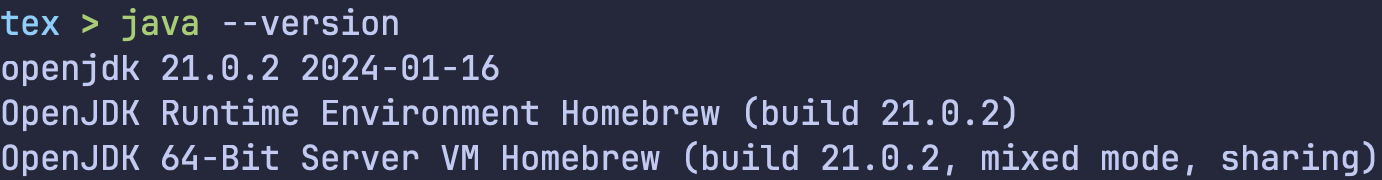
\includegraphics[width=0.9\textwidth]{images/task-1/1.png}
  \caption{Проверка установки среды Java}
  \label{fig:task-1-1}
\end{figure}

\subsection*{Упражнение 2. Создание первой программы}

Для выполнения данного упражнения были созданы два файла с содержимым,
показанным на рисунках \ref{fig:task-2-1} и \ref{fig:task-2-2}.

\begin{figure}[H]
  \inputminted{java}{../code/task-2/TestGreeting.java}
  \caption{Содержимое файла TestGreeting.java}
  \label{fig:task-2-1}
\end{figure}

\begin{figure}[H]
  \inputminted{java}{../code/task-2/Greeting.java}
  \caption{Содержимое файла Greeting.java}
  \label{fig:task-2-2}
\end{figure}

После этого, с помощью команды, показанной на рисунке \ref{fig:task-2-3}, данные
файлы были скомпилированы. После компиляции в папке появились еще два файла:
\foreignlanguage{english}{TestGreeting.class} и
\foreignlanguage{english}{Greeting.class}.

\begin{figure}[H]
  \centering
  \begin{minted}{sh}
    javac TestGreeting.java
  \end{minted}
  \caption{Команда для компиляции исходного кода}
  \label{fig:task-2-3}
\end{figure}

Для выполнения скомпилированного кода была выполнена команда, показанная на
рисунке \ref{fig:task-2-4}. После ее выполнения скомпилированная программа была
запущена и на экран была выведена строка <<Hello>>.

\begin{figure}[H]
  \centering
  \begin{minted}{sh}
    java TestGreeting
  \end{minted}
  \caption{Команда для выполнения скомпилированного кода}
  \label{fig:task-2-4}
\end{figure}

После этого, согласно упражнению, оба класса из ранее приведенных файлов были
перенесены в один файл. При этом класс \foreignlanguage{english}{Greeting} был
объявлен без модификатора \foreignlanguage{english}{public}. На рисунке
\ref{fig:task-2-5} приведен полный исходный код получившейся программы. В
качестве названия основного класса, чтобы избежать конфликтов, было выбрано
название <<\foreignlanguage{english}{TotalGreeting}>>.

\begin{figure}[H]
  \inputminted{java}{../code/task-2/TotalGreeting.java}
  \caption{Исходный код программы}
  \label{fig:task-2-5}
\end{figure}

\subsection*{Упражнение 3. Создание в NetBeans простейшего приложения Java}

В данном упражнении необходимо с помощью интегрированной среды разработки
NetBeans создать проект Java. В качестве категории проекта была выбрана категория
\foreignlanguage{english}{Java with Ant}, а в качестве типа проекта ---
\foreignlanguage{english}{Java Application} (рисунок \ref{fig:task-3-1}). Затем,
для проекта, как показано на рисунке \ref{fig:task-3-2}, было указано имя и
расположение на диске. После нажатия на кнопку
<<\foreignlanguage{english}{Finish}>> было открыто окно NetBeans с редактором
кода (рисунок \ref{fig:task-3-3}).

\begin{figure}[H]
  \centering
  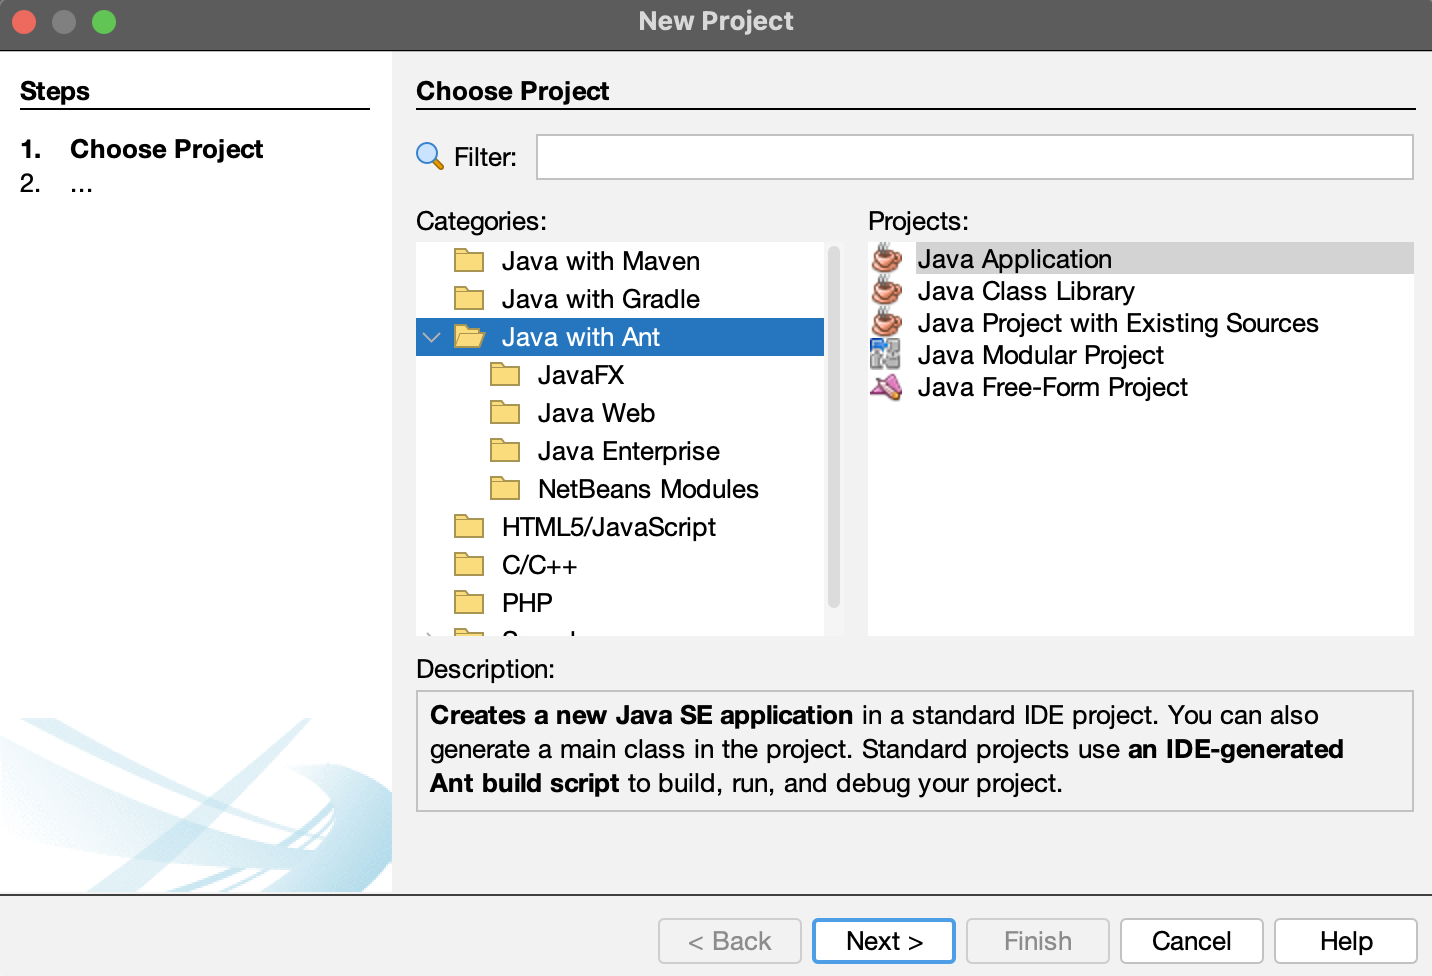
\includegraphics[width=0.6\textwidth]{images/task-3/1.png}
  \caption{Выбор типа проекта}
  \label{fig:task-3-1}
\end{figure}

\begin{figure}[H]
  \centering
  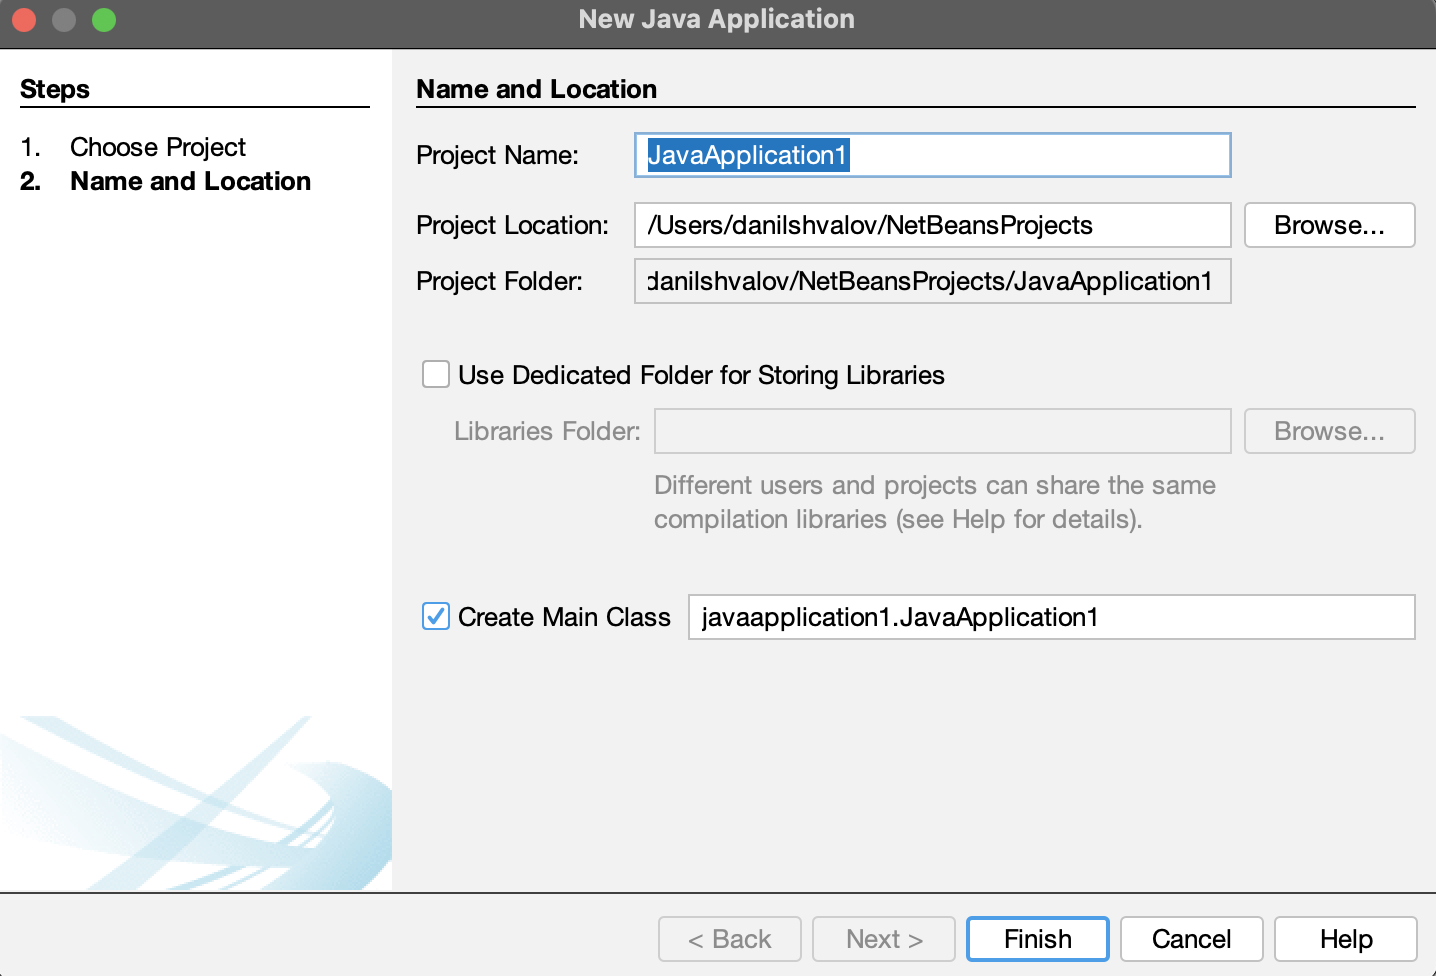
\includegraphics[width=0.6\textwidth]{images/task-3/2.png}
  \caption{Выбор названия проекта}
  \label{fig:task-3-2}
\end{figure}

\begin{figure}[H]
  \centering
  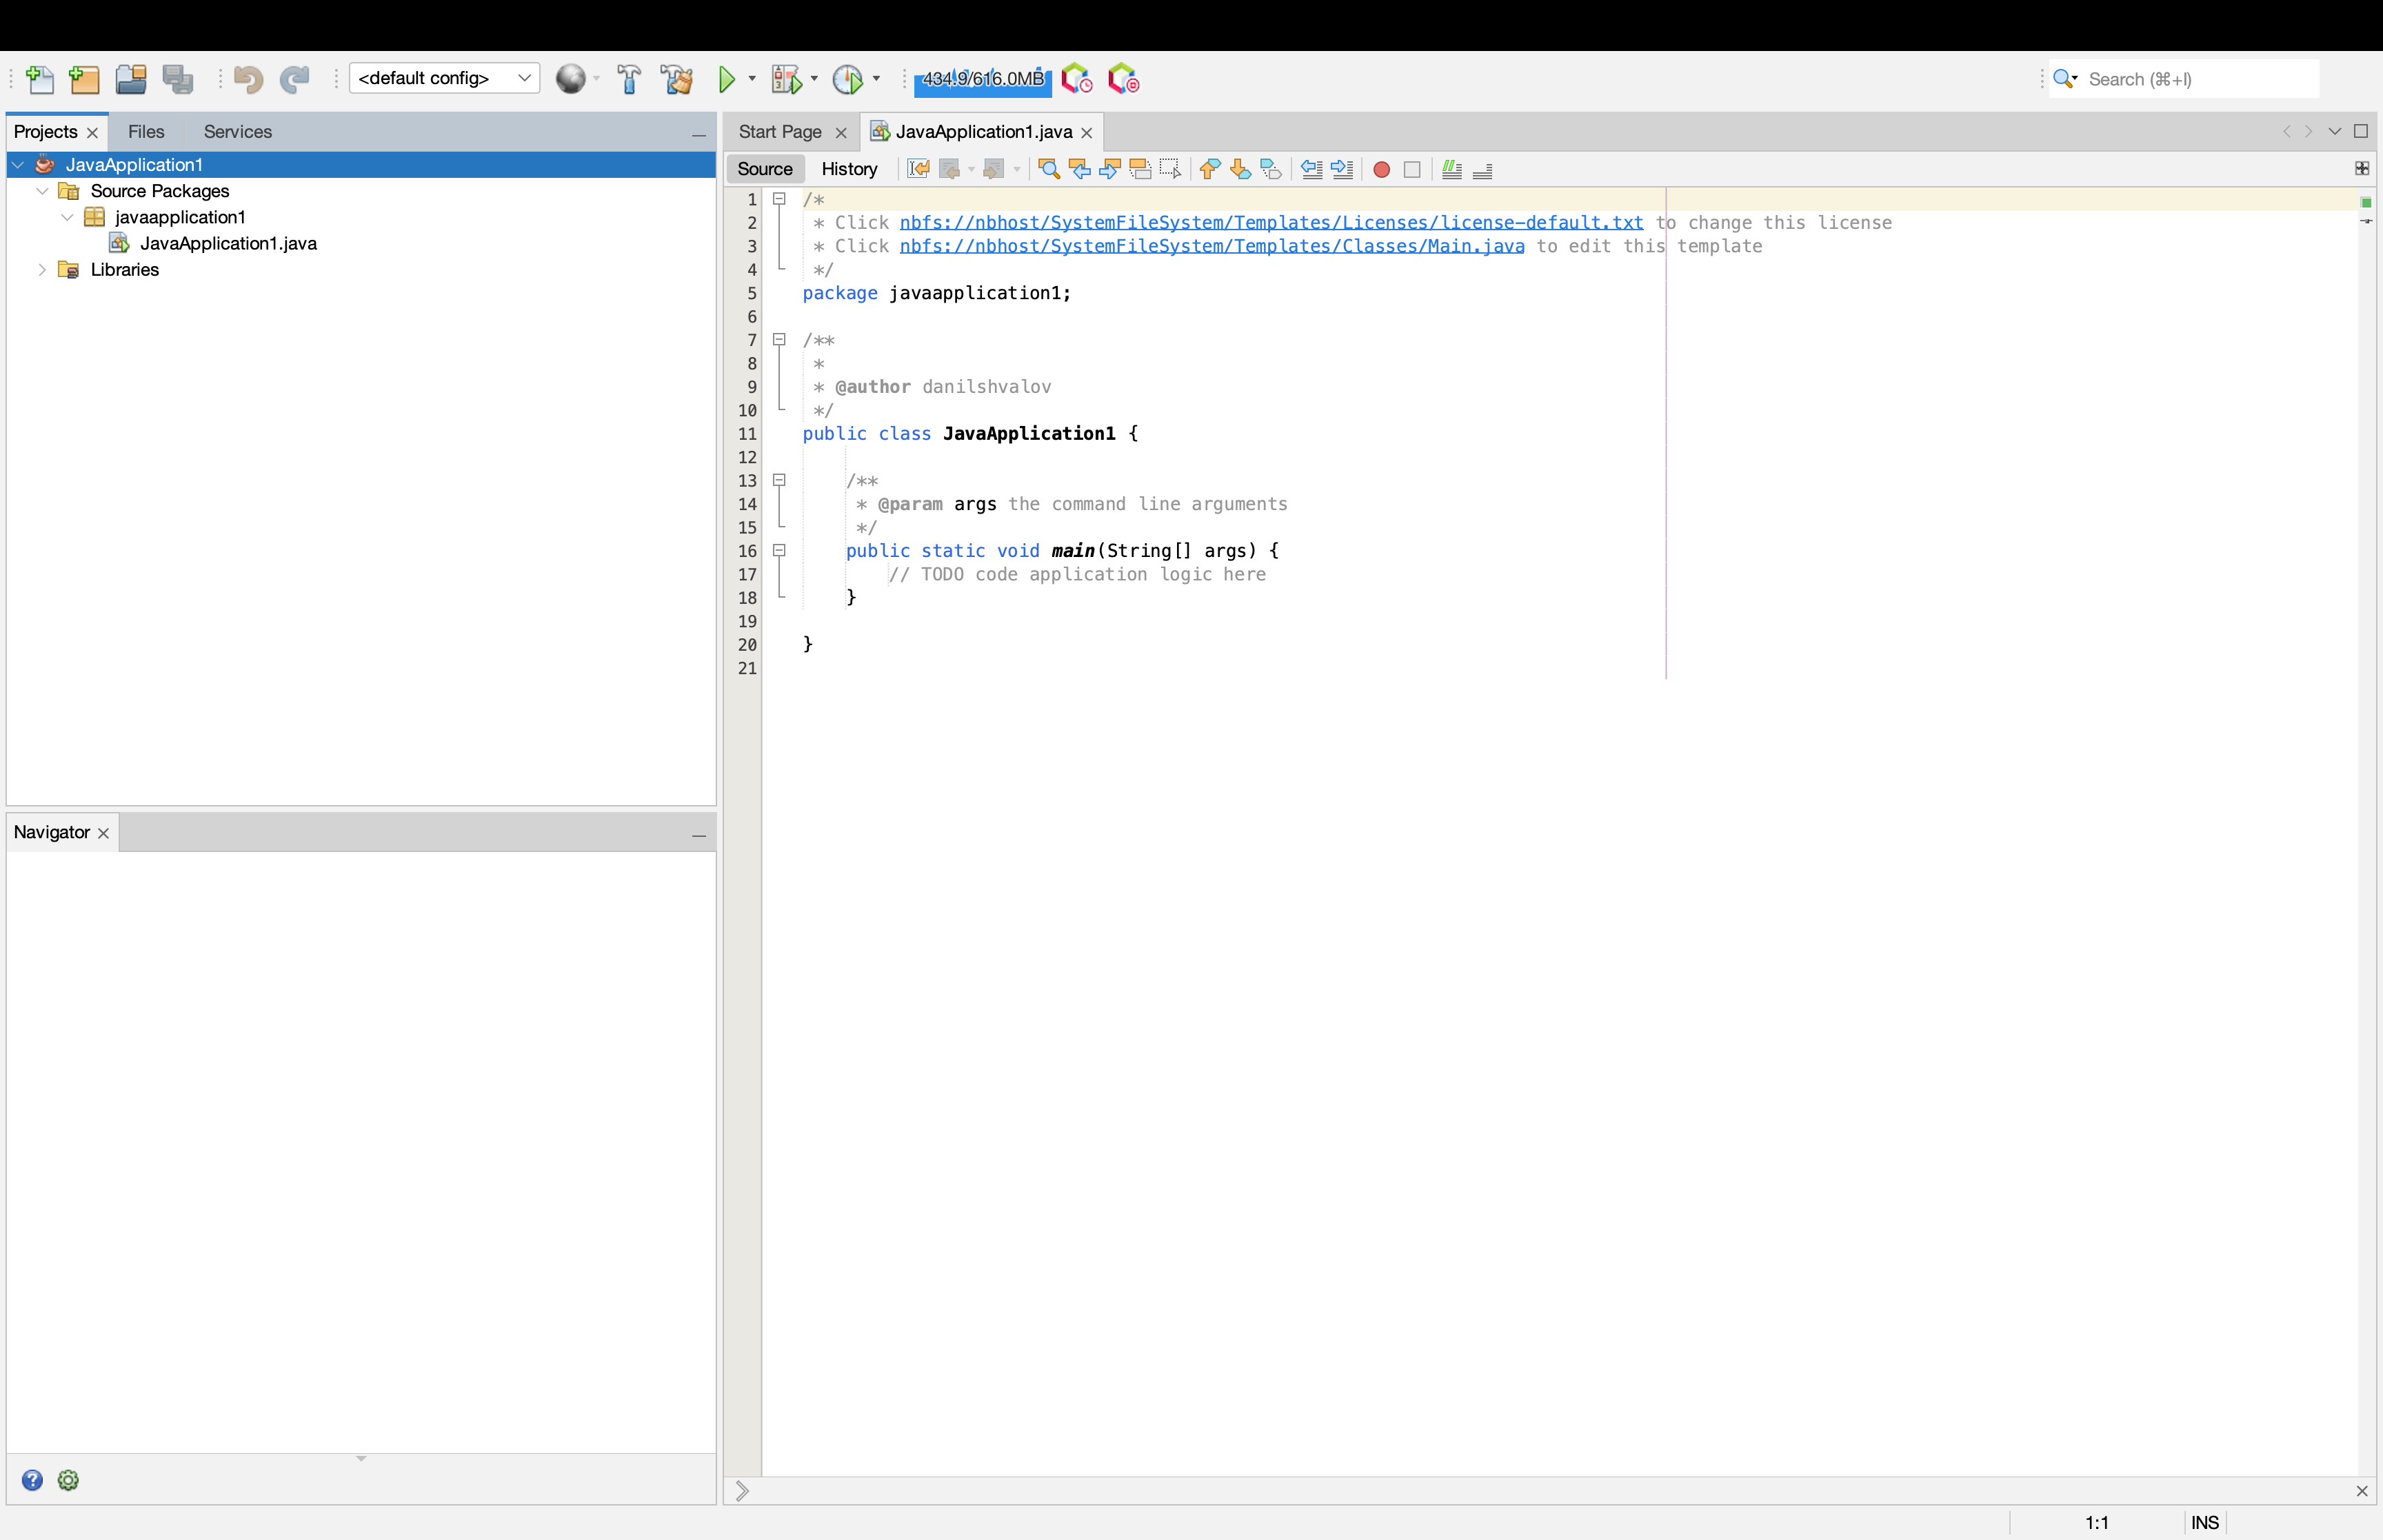
\includegraphics[width=\textwidth]{images/task-3/3.png}
  \caption{Окно проекта NetBeans}
  \label{fig:task-3-3}
\end{figure}

После создания проекта в окне редактора кода, как было показано на рисунке
\ref{fig:task-3-3}, находится шаблон программы. В рамках данного упражнения, в
функцию \foreignlanguage{english}{main} были дописаны строки, показанные на
рисунке \ref{fig:task-3-4}.

\begin{figure}[H]
  \centering
  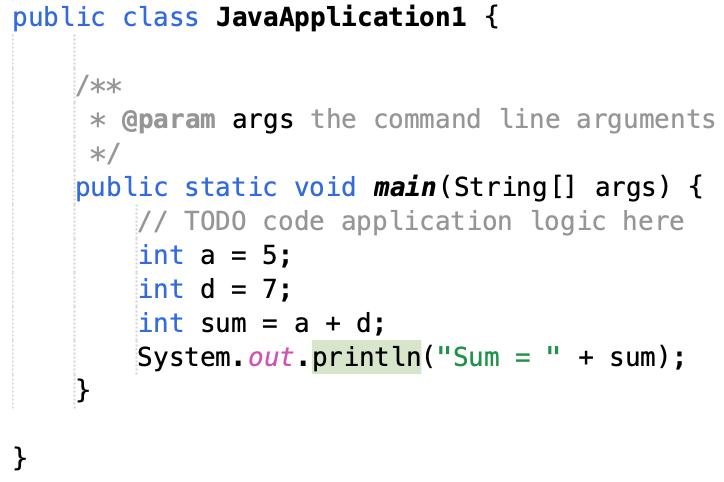
\includegraphics[width=0.7\textwidth]{images/task-3/4.png}
  \caption{Полученная программа}
  \label{fig:task-3-4}
\end{figure}

\subsection*{Упражнение 4. Компиляция файлов проекта и запуск приложения}

С помощью кнопок, показанных на рисунке \ref{fig:task-4-1}, проект был собран.
Также, с помощью кнопки, изображенной на рисунке \ref{fig:task-4-2}, для проекта
была сгенерирована документация. После генерации была открыта страница, которая
показана на рисунке \ref{fig:task-4-3}. Также с помощью кнопки, показанной на
рисунке \ref{fig:task-4-4}, был скомпилирован отдельный файл с программой.

\begin{figure}[H]
  \centering
  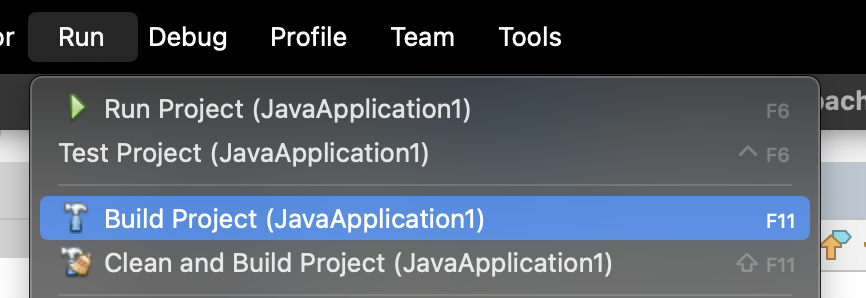
\includegraphics[width=0.5\textwidth]{images/task-4/1.png}
  \caption{Кнопки сборки проекта}
  \label{fig:task-4-1}
\end{figure}

\begin{figure}[H]
  \centering
  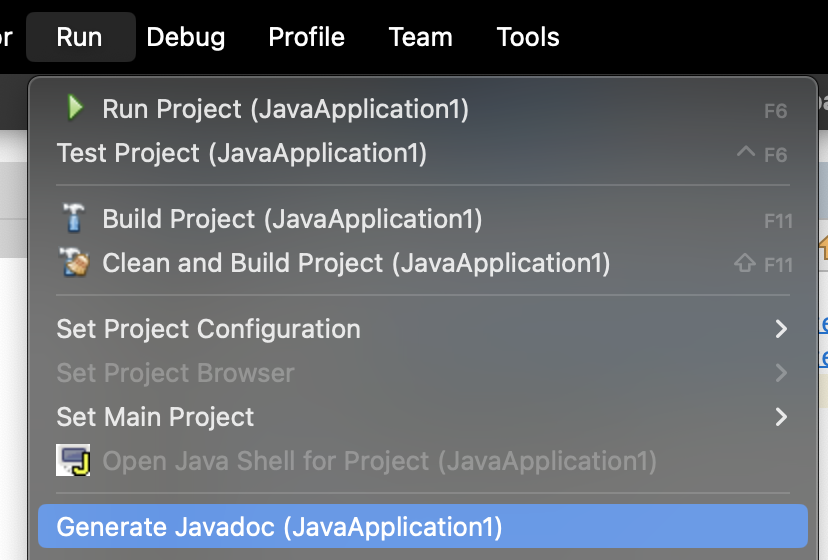
\includegraphics[width=0.5\textwidth]{images/task-4/2.png}
  \caption{Кнопки генерации документации}
  \label{fig:task-4-2}
\end{figure}

\begin{figure}[H]
  \centering
  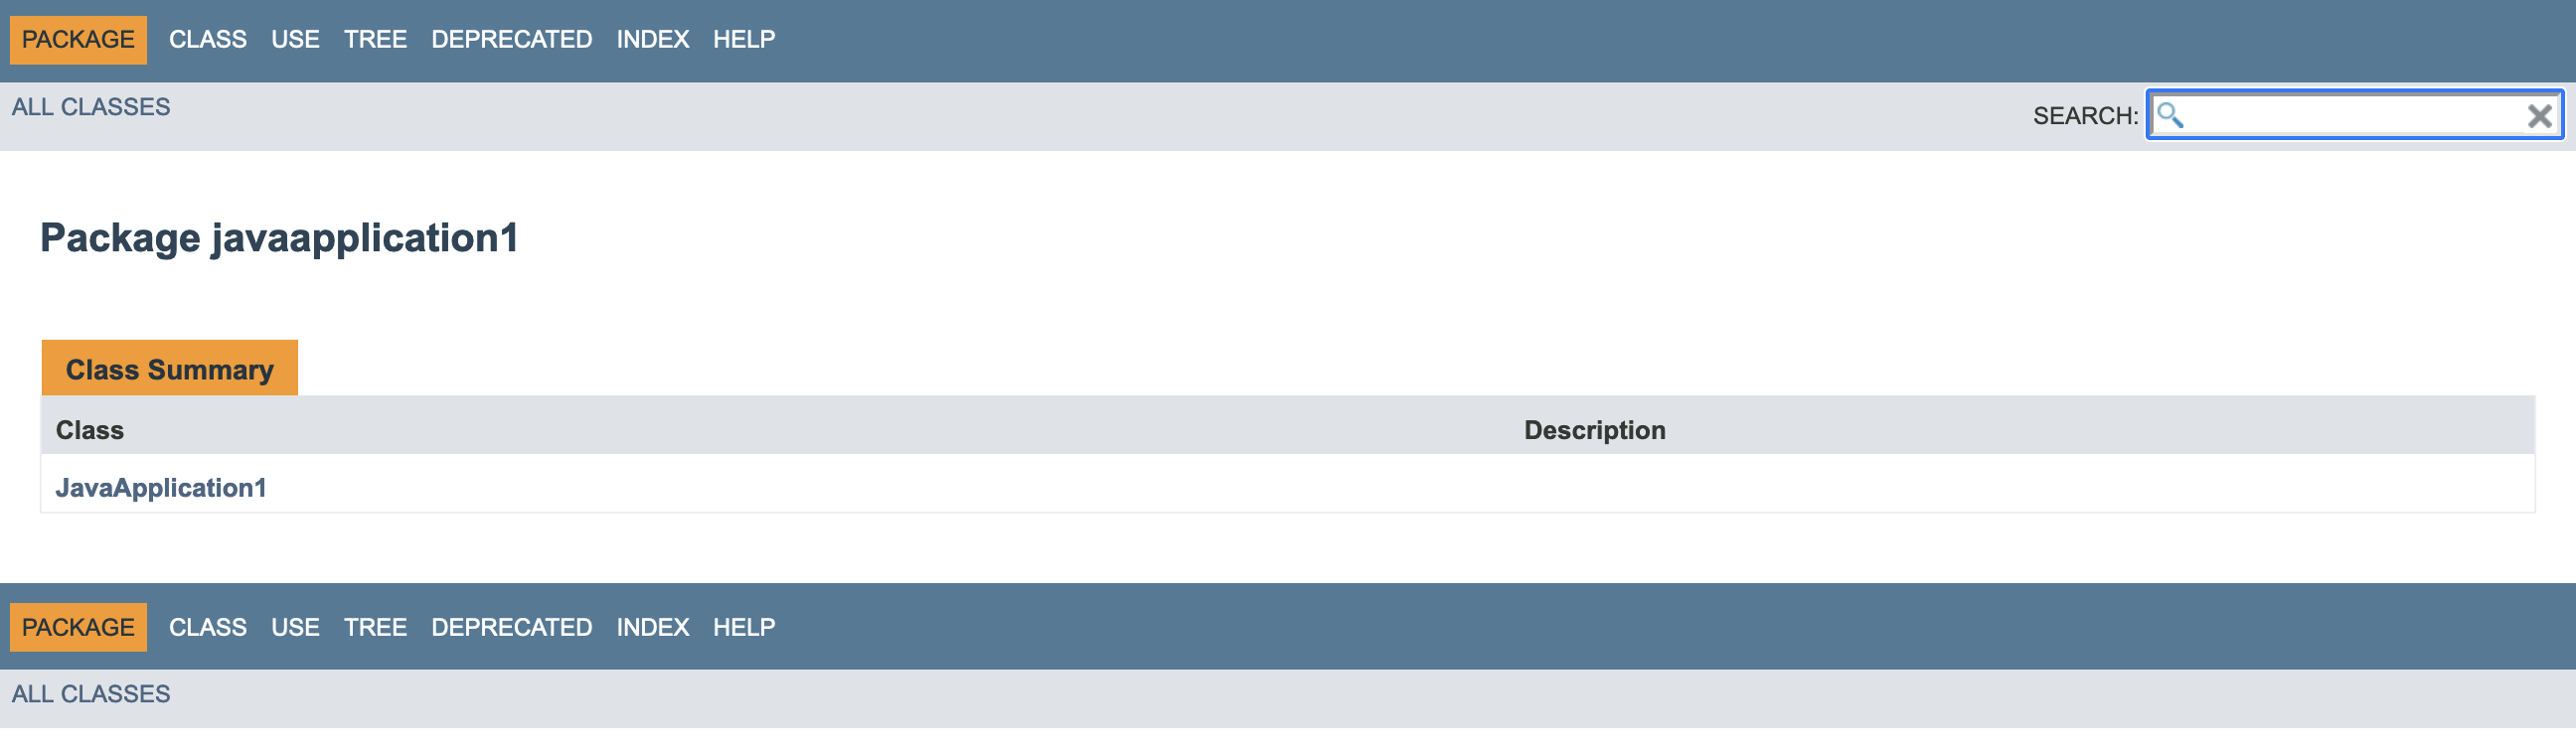
\includegraphics[width=\textwidth]{images/task-4/3.png}
  \caption{Сгенерированная страница документации}
  \label{fig:task-4-3}
\end{figure}

\begin{figure}[H]
  \centering
  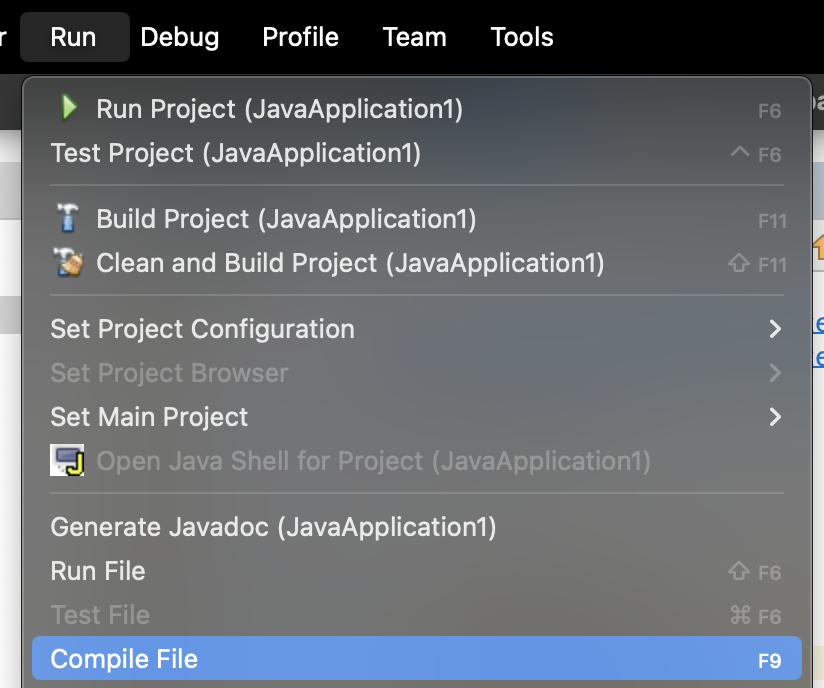
\includegraphics[width=0.5\textwidth]{images/task-4/4.png}
  \caption{Кнопка компиляции файла}
  \label{fig:task-4-4}
\end{figure}

С помощью кнопки, показанной на рисунке \ref{fig:task-4-5}, программа была
запущена. На рисунке \ref{fig:task-4-6} изображен вывод программы.

\begin{figure}[H]
  \centering
  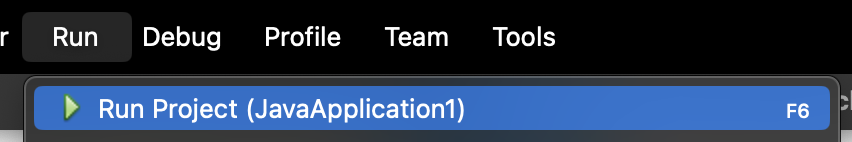
\includegraphics[width=0.5\textwidth]{images/task-4/5.png}
  \caption{Кнопка запуска проекта}
  \label{fig:task-4-5}
\end{figure}

\begin{figure}[H]
  \centering
  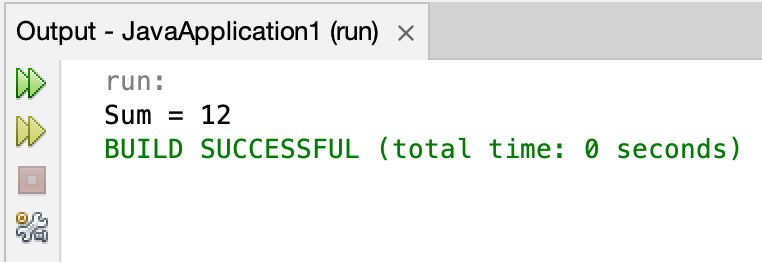
\includegraphics[width=0.5\textwidth]{images/task-4/6.png}
  \caption{Вывод программы}
  \label{fig:task-4-6}
\end{figure}

На рисунке \ref{fig:task-4-7} приведена структура проекта.

\begin{figure}[H]
  \centering
  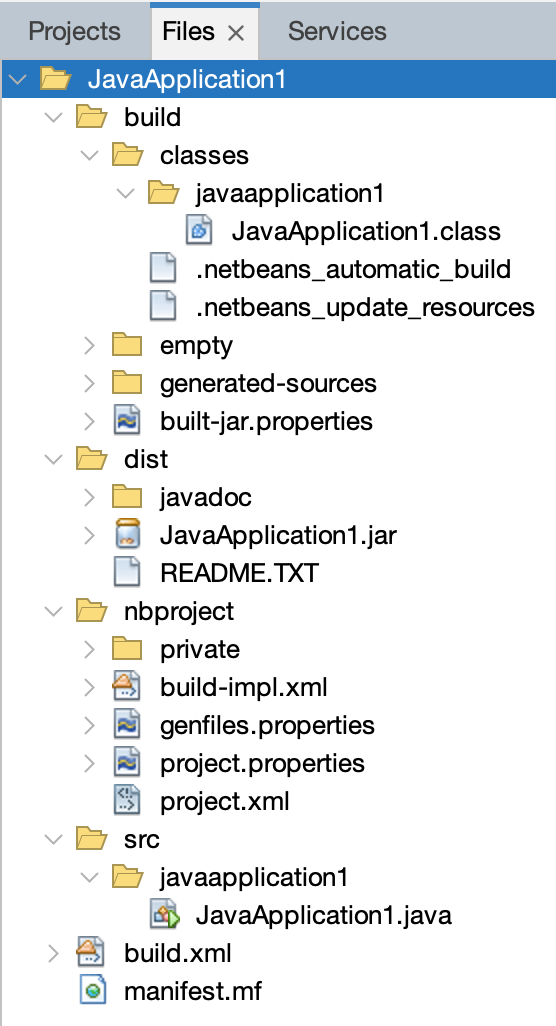
\includegraphics[width=0.35\textwidth]{images/task-4/7.png}
  \caption{Структура проекта}
  \label{fig:task-4-7}
\end{figure}

\section*{Заключение}

В ходе выполнения данной лабораторной работы была установлена среда Java,
создана и скомпилирована первая программа на языке Java. Также была настроена и
изучена интегрированная среда разработки NetBeans: в ней был создан учебный
проект, с помощью которого было изучено, как компилировать код и какая структура
файлов используется в проектах NetBeans.

Цель, поставленная в начале работы, достигнута, задачи выполнены.

\end{document}
